\documentclass{article}
\usepackage{amsmath}
\usepackage{graphicx}
\usepackage{geometry}
\usepackage{hyperref}

\title{Lecture 2 Project: Document Distance}
\author{Yanuar Heru Prakosa}
\date{31-05-2021}

\begin{document}
    \maketitle

    \section*{The Document Distance}
    The assignment from the Lecture 2 in 6-006 is related to one called document distance. 
    Thus I need to find out first what is exactly document distance is.  
    \href{http://6.006.scripts.mit.edu/~6.006/spring08/wiki/index.php?title=Document_Distance_Problem_Definition}{Form this MIT discussion webpage}, I learn that document distance will be measured using vector equations.
    Let D be a text, then a word is a consecutive of alphanumeric characters. 
    We will not distinguish upper case and lower case letters, but we use non alphanumeric characters as delimiter between words.
    For example the word "can't" consist of 2 words: can and t.
    
    Okay now we go to the formulation:
    The word \emph{word frequency distribution} of a document D ia a mapping from words \emph{w} to their frequency count, denoted as $D(w)$.
    We can view the frequency distribution D as vector, with one component per possible word. Each component will be a non-negative integer $\geq 0$.

    The norm of this vector is defined by:
    \begin{equation*}
        N(D) = \sqrt{D \cdot D} = \sqrt{\sum_{w}{D(w)^{2}}}
    \end{equation*}
    Alright this calculation still does not make any sense right now.
    But let's move on, I need to get to how to calculate document distance first.
    Now when we have two documents to be compared to each other, let's name them $D$ and $D'$. 
    The inner product between $D$ and $D'$ is defined as:
    \begin{equation*}
        D \cdot D' = \sum_{w}{D(w)D'(w)}
    \end{equation*}
    So basically this is the sum of products on all word frequencies in two documents.
    Thus, if a word exist 1000 times in one document but never existed in other document the inner product of that part is 0!

    Okay, since our objective is to define distance which is defined here as angle between two documents we need to go back to definition of vector dot products:
    \begin{equation*}
        D \cdot D' = N(D) N(D') cos \theta
    \end{equation*}
    As we looking for an angle we are focusing on $\theta$ right?
    Therefore:
    \begin{equation*}
        cos \theta = \frac{D \cdot D'}{N(D)N(D')}
    \end{equation*}
    \begin{equation*}
        \theta = arccos \left( \frac{D \cdot D'}{N(D)N(D')} \right)
    \end{equation*}
    Deriving from other equations above we will get:
    \[
      \theta = arccos \left( \frac{\sum_{w}{D(w)D'(w)}}{\sqrt{\sum_{w}{D(w)^{2}}} \sqrt{\sum_{w}{D'(w)^{2}}}}\right)  
    \]
    From those formula we can infer that if both Documents are the same then the $angle(D,D') = \theta = 0$.
    On the other hand if both documents are completely different in the sense there are no similarity in terms of word used in it then the $angle(D,D') = \theta = \frac{\pi}{2}$. Please note we are using \emph{radians} in this matter.

    \section*{Pre Example}
    To make it clearer I think a simple practical example is mandatory. 
    Let us have two sentences that we will use as documents. 
    One is "To be or not to be" and the other is "Doubt truth to be a liar". 
    We will calculate the distance between these two documents.

    Now we already list all unique set of words and it can be seen in this table plus its frequencies:
    \begin{center}
        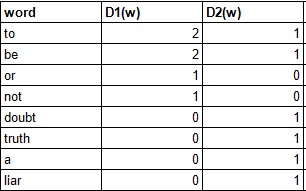
\includegraphics{table word frequencies}    
    \end{center}
        
    Now let's get back to the formula: 
    \[
      \theta = arccos \left( \frac{\sum_{w}{D(w)D'(w)}}{\sqrt{\sum_{w}{D(w)^{2}}} \sqrt{\sum_{w}{D'(w)^{2}}}}\right)  
    \]
    we begin with the denominator part first.

    \newpage
    To calculate the denominator we need to find $\sum_{w}{D(w)^{2}}$ and $\sum_{w}{D'(w)^{2}}$ first. Here is the results of the calculation:
    \begin{center}
        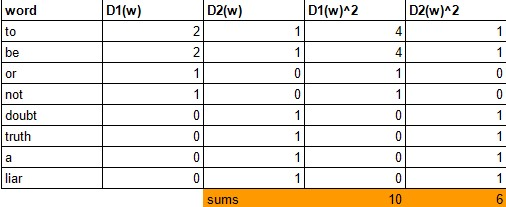
\includegraphics{square frequencies table.jpg}
    \end{center}

    As you can see the sums already being included in the table above.
    We can use it as our denominators, but remember those sum products must be subject to a square root operations.
    Now we need to calculate the nominator side: $sum{D(w)D'(W)}$, which we have already calculated also using spreadsheet:
    \begin{center}
        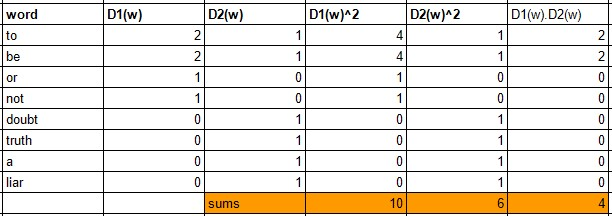
\includegraphics[scale=0.8]{inner product sum table.jpg}
    \end{center}

    As you can see on the table above the $sum{D(w)D'(W)} = 4$, now we can put all of them in the formula:
    \[\theta = arccos \left( \frac{4}{\sqrt{10} \sqrt{6}}\right)\]
    \[\theta = arccos \left( \frac{4}{\sqrt{10.6}}\right)\]
    \[\theta = arccos\left( 0.52\right)\]
    \[\theta = 1.028157225\]

    There you are, that is in summary how we will measure the distance between to documents. 

    \section*{Summary}
    Here is what you should do when measuring the distance between two documents:
    \begin{enumerate}
        \item list all words in a set, meaning there are no double words in a set all words are unique
        \item count the frequency of occurance for each word in each document (WARNING: EACH NOT TOTAL)
        \item use vector inner product and normalization also dot products to calculate the angle (SEE THE FORMULAS AND EXAMPLE ABOVE)
        \item that angle when is closer to 0 (the minimum angle is 0) then the chance both documents are the same is higher (some use this as an indication of plagiarism)
        \item Vice versa when the angle is closer towards $\frac{\pi}{2}$ then the documents are less similar.
        \item Just remember this is only a basic algorithm on how to measure document distance, many ways can be used to cheat this algorithm thus this kind of measurements always evolving in terms of algorithms. 
        \item Stay tune and keep learning!
    \end{enumerate}

\end{document}